\documentclass{article}
\usepackage{hyperref}
\usepackage[table]{xcolor}
\usepackage{listings}
\usepackage{lmodern}
\usepackage[left=0.25in, right=0.25in, top=0.75in, bottom=0.75in]{geometry}
\usepackage{graphicx}
\usepackage{amsmath,amssymb}
\usepackage{tikz}
\usepackage{pgfplots}
\usepackage{subfigure}
\usepackage{enumerate}
\usepackage{tcolorbox}
\usepackage{fancyhdr}
\usepackage{cancel}
\usepackage{placeins}
\usepackage{multirow}
\usepackage{algorithm2e}
\pagecolor{white}
\color{black}

\pagestyle{fancy}

\hypersetup{%
  colorlinks=true,% hyperlinks will be black
  linkbordercolor=red,% hyperlink borders will be red
  pdfborderstyle={/S/U/W 1}% border style will be underline of width 1pt
}

\newcommand{\soln}{\\ \textbf{Solution}: }
\newcommand{\bkt}[1]{\left(#1\right)}

\lhead{MA5892: Numerical Methods and Scientific Computing}
\chead{Assignment: 5}
\rhead{Rollnumber: PH15M015}

\begin{document}
\begin{enumerate}
\item Prove the Equioscillation theorem.

\textbf{Equioscillation theorem:} Let $f \in C[-1,1]$ and $p(x)$ be a polynomial whose
degree doesn't exceed $n$. $p$ minimizes $\lVert f-p \rVert_{\infty}$ iff $f-p$ 
equioscillates at $n+2$ points. \\

\textbf{Proof:}

Let us define the supremum norm of $f$ to be:

\begin{equation*}
\lVert f \rVert = sup \{f(x): x \in [a, b] \}
\end{equation*}

and the best minimax error of degree $n$ by
$d_{n} = \inf\{ \lVert f - p \rVert $: $p$ is a polynomial on $[a,b]$ of degree $\leq n$\}


The theorem is trivially true if $f$ is itself a polynomial of degree $<= n$. We assume
not, and so $d_{n} > 0$. \\

Since $f$ be continuous on $[-1, 1]$, and let $p$ be a polynomial of degree $<= n$. If $f,
\ p$ has a non-uniform alternating set $X = (x_{0},...,x_{n+1})$ of length $n+2$, then 
$d_{n} \geq min \{|e_{i}|: i = 0, 1, ..., n+1 \}$. \\

Suppose that $f,\ p_{n}$ has an alternating set of length $n+2$.
We have $\lVert f - p_{n} \rVert \leq d_{n}$. As $d_{n} \leq \lVert f - p_{n} \rVert$ by
the definition of $d_{n}$, it follows that $p_{n}$ is a polynomial of best approximation 
to $f$. \\

Now suppose that $p_{n}$ is a polynomial of best approximation to $f$ and $f \neq p$. Then
$f,\ p_{n}$ has an alternating set of length $2$m and it can be extended into a sectioned
alternating set of length $m$. We must have $m \geq n + 2$, for if $m \leq n+1$ then we
could add a polynomial $q$ of degree $\leq n$ to $p_{n}$ and get a better approximation
than $p_{n}$, which is impossible. Thus every polynomial of best approximation has an
alternating set of length at least $n + 2$. \\

To show uniqueness, suppose that $p_{n}$ and $q_{n}$ are both polynomials of best
approximation, and we will show that they are equal. \\

Note that $(p_{n} + q_{n})/2$ is a polynomial of best approximation, as:

\begin{equation*}
\bigg \lVert f - \frac{p_{n} + q_{n}}{2} \bigg \rVert = \bigg \lVert \frac{f - p_{n}}{2} +
    \frac{f - q_{n}}{2} \bigg \rVert \leq \frac{1}{2} \lVert f - p_{n} \rVert + \frac{1}{2} \lVert f - q_{n} \rVert = d_{n}
\end{equation*}

Therefore, there are $n+2$ alternating points at which $(f - p_{n})/2 + (f - q_{n})/2 = \pm d_{n}$. \\

At each of these alternating points, $f - p_{n}$ and $f - q_{n}$ are both $d_{n}$ or both 
$-d_{n}$. So $f - p_{n}$ and $f - q_{n}$ agree on $n + 2$ points, and so 
$(f - p_{n}) - (f - q_{n}) = q_{n} - p_{n} = 0$ at these $n + 2$ points. Since
$q_{n} - p_{n}$ is a polynomial of degree $\leq n$, $q_{n}$ and $p_{n}$ must be identical.
Therefore the polynomial $p_{n}$ of best approximation is unique. \\


\item Consider the function $f(x) = |x|$ on the interval $[-1,1]$.
\begin{itemize}
\item Prove that of all polynomials whose degree doesn't exceed $3$, $p(x) = x^{2} +
\displaystyle \frac{1}{8}$ is the best approximation in the $\lVert \cdot \rVert_{\infty}$ norm.
\item Interpolate the function using $4$ Legendre nodes and Chebyshev nodes. Call the
polynomials obtained as $p_{L}(x)$ and $p_{C}(x)$.
\item Fill in the table below. You should be able to complete the table by hand.
\end{itemize}

\begin{table}[ht]
\centering
\begin{tabular*}{.3\linewidth}{@{\extracolsep{\fill}}|c|c|c|}
\hline
Approximation & $\lVert \cdot \rVert_{2}$ & $\lVert \cdot \rVert_{\infty}$ \\
\hline
$f(x) - p(x)$ & & \\
\hline
$f(x) - p_{L}(x)$ & & \\
\hline
$f(x) - p_{C}(x)$ & & \\
\hline
\end{tabular*}
\end{table}

Comment on the errors you obtain using the different norm. Which one is optimal under the
$\lVert \cdot \rVert_{2}$ and $\lVert \cdot \rVert_{\infty}$? For each norm, order the different approximations in increasing order of accuracy.

\item \textbf{Error estimate of Gaussian quadrature:} Prove that
\begin{equation*}
\int_{a}^{b} w(x) f(x) dx - \sum_{i=1}^{n} w_{i} f(x_{i}) = \frac{f^{(2n)} (\xi)}{(2n)!} \lVert p_{n} (x) \rVert_{w}^{2}
\end{equation*}

for some $\xi \in (a,b)$ and $p_{n}(x)$ is the monic orthogonal polynomial corresponding to the weight function $w(x)$.

\item Let $f(x)$ be periodic function on $[0,1]$ of the form 
\begin{equation*}
f(x) = a_{0} + \sum_{k=1}^{n} (a_{k}\ cos(2k\pi x) + b_{k}\ sin(2k\pi x))
\end{equation*}

Take the case of $n = 20$ and $a_{k}, b{k}$ are uniformly distributed on $[-1,1]$.
Approximate $\displaystyle \int_{-1}^{1} f(x) dx$ using trapezoidal rule with $k$ points where $k \in
\{1,2,...,80\}$. Compare the error with the exact integral and comment on the result you
obtain. Prove that the trapezoidal rule give you the exact integral for $k > n$.

\textbf{Program:}
\lstinputlisting[language=Python]{Python/trapezoidal.py}

\item Evaluate $\displaystyle \int_{-1}^{1} e^{-x^{2}} dx$ using Gaussian quadrature with $n$ nodes,
where $n \in \{3,4,5,...,51\}$. Plot the absolute error as a function of $N$ on a log-log
plot.

\textbf{Program:}
\lstinputlisting[language=Python]{Python/gaussleg.py}

%figure_1
\begin{figure}[ht!]
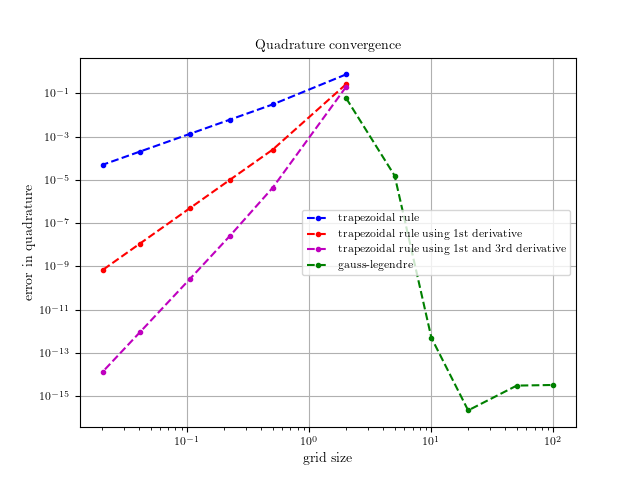
\includegraphics[width=20cm,height=12cm,keepaspectratio]{Python/gaussleg.pdf}
\centering
\end{figure}

\end{enumerate}
\end{document}
